\section{Einleitung}

Machine Learning stellt einen Aspekt der künstlichen Intelligenz dar, der in der vergangenen Zeit an immer größerer
Bedeutung gewonnen hat. In diesem Kontext ist insbesondere das Deep Learning hevorzuheben, das wiederum einen Teilbereich
des Machine Learnings darstellt. Dessen Popularität lässt sich zum Einen damit erklären, dass es die Geschwindigkeit und
Reife heutiger Prozessoren (CPU/GPU/TPU\footnote{Wikipedia, Tensor Processing Unit.\newline
(https://de.wikipedia.org/wiki/Tensor\_Processing\_Unit)}/FPGA\footnote{Wikipedia, Field Programmable Gate Array.\newline
(https://de.wikipedia.org/wiki/Field\_Programmable\_Gate\_Array)})
zulässt Ergebnisse in akzeptabler Zeit zu erzielen und zum Anderen damit, dass durch das stetige Anwachsen der durchs Internet
erzeugten Daten, genug Material zur Verfügung steht, mit dem gearbeitet werden kann. Besonders im Kontext von Bilderkennungen
und Klassifizierungsproblemen sind Techniken des Machine Learnings kaum noch wegzudenken.

In bildgebenden Medien, Videos wie Fotos, werden Gesichter von Menschen verfälscht, um deren Identität unkenntlich
zu machen.\footnote{Andrew Senior, Protecting Privacy in Video Surveillance, S 130 ff.\label{fn:protecting_privacy}}
Diese Technologien werden von
öffentlichen Medien, wie Privatpersonen verwendet. In der Vergangenheit
gab es den Fall eines Kinderschänders, der verfälschte Gesichtsbilder von sich veröffentlichte. Er verwendete dabei
ein Verfahren, das Pixel um einen zentralen Punkt zu einer Spirale rotiert. Behörden war es damals möglich, diese
Form der Gesichtsverfälschung, deren Informationsverlust im Vergleich zu den Verfahren, die in dieser Arbeit behandelt
werden, gering ist, aufzuheben und das Gesicht weitgehends wiederherzustellen.
\footnote{Wikipedia, ``Christopher Paul Neil''.\newline(https://en.wikipedia.org/wiki/Christopher\_Paul\_Neil)}
Motiviert unter anderem dadurch,
stellt diese Arbeit eine Grundlagenanalyse dar, in wie weit CNNs dafür verwendet werden können sehr viel verbreitetere,
aber destruktive Obfuscation-Verfahren anzugreifen.

Maßgeblich kommen beim Verfälschen zwei Verfahren zum Einsatz\textsuperscript{\ref{fn:protecting_privacy}}:
``Weichzeichnen'' (Gaussian Blur)\footnote{Wikipedia, Gaussian Blur.\newline(https://en.wikipedia.org/wiki/Gaussian\_blur)}
 und ``Verpixelung'' (Pixelization)\footnote{Wikipedia, Pixelization.\newline(https://en.wikipedia.org/wiki/Pixelization)\label{label:pixelization}}.


\subsection{Weichzeichnen}
Der gaußsche Weichzeichner oder \textit{Gaussian Smoothing}, beschreibt ein Verfahren, mit dem der Kontrast von Bildern
verringert wird. Damit wird der Verlust von Detailinformationen erreicht. Die mathematische Formel, nach der die
Transformation funktioniert, lautet:

\parskip\baselineskip

\begin{figure}[h]
    \centering
    \(G(x) = \frac{1}{\sqrt{2 \pi \sigma^2}} e^{-\frac{x^2}{2 \sigma^2}}\)
    \caption{Gleichung der gausschen Weichzeichnung zweier Dimensionen.}
    \label{fig:func-blur}
\end{figure}


\par
\par

\textit{x} und \textit{y} beschreiben die Distanz zum Ursprung der jeweiligen Achse, \textit{\(\sigma\)} ist ein Parameter der Funktion, der
beschreibt wie sehr die Weichzeichnung streut (siehe Abbildung \space \vref*{fig:gaussianBlur}).
Der Formel kann man entnehmen, dass die
Farbinformationen benachbarter Pixel in das Ergebnis des aktuell zu berechnenden Pixels miteinfließen. Hier werden
die Informationen verschiedener Pixel auf den selben Wertebereich eines Pixels abgebildet. Der dadurch entstehende
Informationsverlust ist irreversibel.

\captionsetup[subfigure]{labelformat=empty, labelsep=none}
\begin{figure}[h]
    \centering
    \begin{subfigure}{0.3\textwidth}
        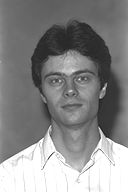
\includegraphics[width=0.9\textwidth]{introduction_blur_original}
        \caption{\small Original}
    \end{subfigure}
    \begin{subfigure}{0.3\textwidth}
        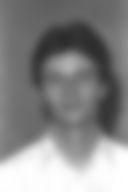
\includegraphics[width=0.9\textwidth]{introduction_blur_sigma_3}
        \caption{\small \(\sigma = 3\)}
    \end{subfigure}
    \begin{subfigure}{0.3\textwidth}
        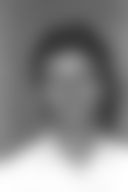
\includegraphics[width=0.9\textwidth]{introduction_blur_sigma_6}
        \caption{\small \(\sigma = 6\)}
    \end{subfigure}

    \caption{Vergleichsbild Weichzeichnen mit verschiedenen Parametern.}
    \label{fig:gaussianBlur}
\end{figure}

\subsection{Verpixelung}
Auch Mosaic-Verfahren, meint eine Menge an Verfahren, die die Auflösung von Bildern oder Bereiche derer künstlich
verringern, um Detailinformationen zu verbergen. Hierfür wird der unkenntlich zu machende Bereich in gleichmäßige
Unterbereiche aufgeteilt und deren resultierender Farbwert aus den Pixeln des Ursprungsbildes gemittelt. Bei dieser
Verfahrensfamilie gibt es eine Vielzahl an Variationen, die sich in Größe und Form der Unterbereiche und dem genauen
Algorithmus, der verwendet wird, um die Unterbereiche unkenntlich zu machen, unterscheidet.

\begin{figure}[h]
    \centering
    \begin{subfigure}{0.3\textwidth}
        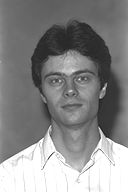
\includegraphics[width=0.9\textwidth]{introduction_mosaic_original}
        \caption{\small Original}
    \end{subfigure}
    \begin{subfigure}{0.3\textwidth}
        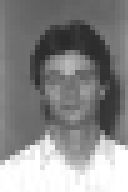
\includegraphics[width=0.9\textwidth]{introduction_mosaic_5}
        \caption{\small Kantenlänge 5px}
    \end{subfigure}
    \begin{subfigure}{0.3\textwidth}
        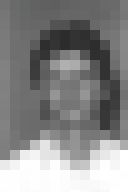
\includegraphics[width=0.9\textwidth]{introduction_mosaic_10}
        \caption{\small Kantenlänge 10px}
    \end{subfigure}

    \caption{Vergleichsbild Weichzeichnen mit verschiedenen Kantenlängen.}
    \label{fig:pixelization}
\end{figure}

Der in diesem Verfahren betrachtete Parameter (siehe Abbildung \space \vref*{fig:pixelization}), entspricht der Kantenlänge der
resultierenden verpixelten Unterbereiche.
